\documentclass[11pt]{report}
\usepackage[spanish]{babel}
\usepackage[utf8]{inputenc}
\usepackage{amsmath}
\usepackage{amssymb}
\usepackage{graphicx}
\usepackage{parskip}
\usepackage{cancel}
\newcommand{\s}{\underline{Soluci\'{o}n:}}
\graphicspath{ {images/} }

\begin{document}{}
\title{Matemáticas para las Ciencias Aplicadas III \\ Tarea 2}
\maketitle

\textbf{Anton-Bivens-Davis} \\

\textbf{Sección 14.2} \\

\textbf{15-18} Evaluate the double integral in two ways using iterated integrals:
(a) viewing $R$ as a type I region, and (b) viewing $R$ as a type II region.

\textbf{18.} \\

$ {\displaystyle \iint \limits_R } \, y \, \, \text dA; \, R$ is the region in
the first quadrant enclosed between the circle $x^2 + y^2 = 25$ and the line
$x + y = 5$. \\

\textbf{19-24.} Evaluate the double integral in two ways using iterated
integrals: \\

\textbf{22.} $ {\displaystyle \iint \limits_R } \, x \, \, \text dA; \, R$
is the region enclosed by $y = sin^{-1} x, x = \frac{1}{\sqrt{2}},$ and $y = 0$.
\\

\s

Entonces $0 \leq y \leq \frac{\pi}{4}$ y $x$ va desde
$x = \sin y$ a $ x = \frac{1}{\sqrt{2}}$  por lo que se tiene
\[{\displaystyle \iint \limits_R } \, x \, \, \text dA; \, R =
\int^{\frac{\pi}{4}}_{0}\int^{\frac{1}{\sqrt{2}}}_{sin y} x dx dy\]
\[\hspace{1.9cm}= \int^{\frac{\pi}{4}}_{0} \frac{x^2}{2} \Big|^{\frac{1}{\sqrt{2}}}_{sin y} dy \]
\[\hspace{4.5cm}= \int^{\frac{\pi}{4}}_{0} \left(\frac{\left(\frac{1}{\sqrt{2}}\right)^2}{2}
- \frac{\left(sin y\right)^2}{2} \right) dy \]
\[\hspace{2.5cm}= \int^{\frac{\pi}{4}}_{0} \frac{1}{4} - \frac{sin^2y}{2} dy\]
\[\hspace{2.8cm}= \frac{1}{4}\int^{\frac{\pi}{4}}_{0} 1 - 2 sin^2y dy\]
\[\hspace{2cm}= \frac{1}{4}\int^{\frac{\pi}{4}}_{0} \cos 2y dy \]
\[\hspace{2.1cm}= \frac{1}{4}\left(\frac{1}{2}\sin2y\Big|^{\frac{\pi}{4}}_{0}\right)\]
\[\hspace{3.6cm}= \frac{1}{8}\left(\sin2\left(\frac{\pi}{4}\right) - \sin2(0)\right)\]
\[\hspace{1.1cm}= \frac{1}{8}\left(1 - 0\right)\]
\[\hspace{-0.1cm}= \frac{1}{8}\]
\textbf{28.} \\


(a) By hand or with the help of a graphing utility, make a sketch of the region
$R$ enclosed between the curves $y = 4x^3 - x^4$ and $y = 3 - 4x + 4x^2$. \\

(b) Find the intersections of the curves in part (a). \\

(c) Find $ {\displaystyle \iint \limits_R } \, x \, \, \text dA $ \\

\textbf{37-38} Use double integration to find the volume of the solid. \\

\textbf{37.} \\

\begin{figure}[h]
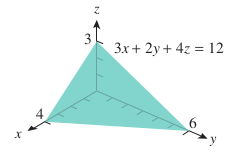
\includegraphics[scale=0.5]{img1.png}
\centering
\end{figure}

\textbf{57.} Try to evaluate the integral with a CAS using the stated order of
integration, and then by reversing the order of integration.\\

Utilizar\'{e} Wolfram Mathematica para evaluar las integrales

(a) $ {\displaystyle \int \limits_0^4 \int \limits_{\sqrt{x}}^2 } \, \sin{\pi y^3} \, \, \text dx \text dy $ \\
\begin{figure}[h]
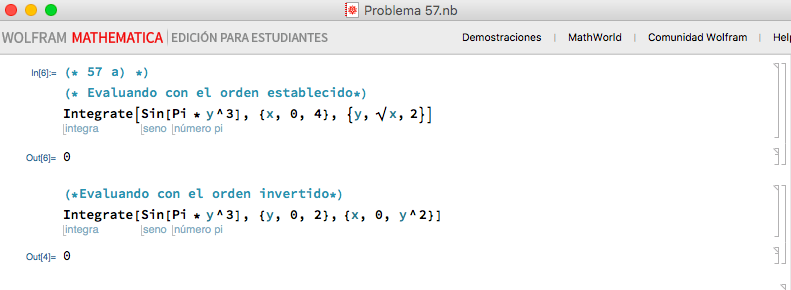
\includegraphics[scale=0.5]{img4.png}
\centering
\end{figure}

Obtuvimos que la integral siguiendo el orden establecido
es $0$ al igual que si invertimos el orden de la integral.

(b) $ {\displaystyle \int \limits_0^1 \int \limits_{sin^{-1}y}^{\frac{\pi}{2}} } \, \sec{\cos{x}}^2 \, \, \text dx \text dy $ \\
\begin{figure}[h]
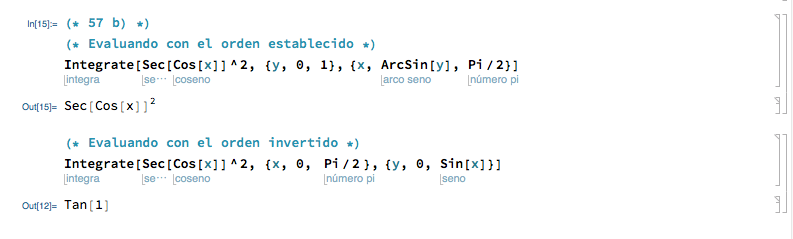
\includegraphics[scale=0.5]{img3.png}
\centering
\end{figure}

La integral siguiendo el orden establecido no se puede calcular en Mathematica,
y la integral invertiendo el orden es $\tan(1)$

\textbf{59.} Evaluate $ {\displaystyle \iint \limits_R } \, xy^2 \, \, \text dA $ over
the region R shown in the accompanying figure. \\
\begin{figure}[h]
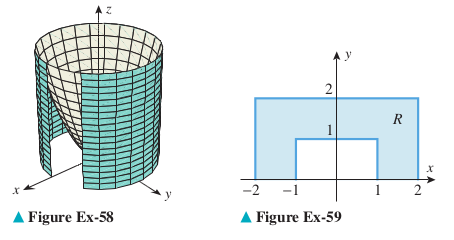
\includegraphics[scale=0.5]{img2.png}
\centering
\end{figure}

\s

Como podemos ver en la figura la podemos dividir en 3 partes
\[1.\, -2 \leq x \leq -1, \, 0 \leq y \leq 2\]
\[2.\, -1 \leq x \leq 1, \, 1 \leq y \leq 2\]
\[3.\, 1 \leq x \leq 2, \, 0 \leq y \leq 2 \]
Entonces
\[{\displaystyle \iint \limits_R } \, xy^2 \, \, \text dA =
\int^{-1}_{-2} \int^{2}_{0} xy^2 \, \text dy \, \text dx +
\int^{1}_{-1} \int^{2}_{1} xy^2 \, \text dy  \, \text dx +
\int^{2}_{1} \int^{2}_{0} xy^2 \, \text dy \, \text dx \qquad (1)\]
Ahora calcularemos cada una de las integrales por separado
\begin{itemize}
\item Calculemos la integral en $ -2 \leq x \leq -1, \, 0 \leq y \leq 2$
\[\int^{-1}_{-2} \int^{2}_{0} xy^2 \, \text dy \, \text dx
= \int^{-1}_{-2} \left(\frac{xy^3}{3}\right)\Big|^{2}_{0} \, \text dx \]
\[\hspace{2.05cm}= \int^{-1}_{-2} \frac{8x}{3} \, \text dx \]
\[\hspace{2.1cm}= \frac{8}{3} \int^{-1}_{-2} x \, \text dx \]
\[\hspace{2.2cm}= \frac{8}{3} \left(\frac{x^2}{2}\right)\Big|^{-1}_{-2} \]
\[\hspace{1.65cm}= \frac{8}{\cancel{3}}\left(-\frac{\cancel{3}}{2}\right)\]
\[\hspace{0.6cm}= -4\]

\item Calculemos la integral en $-1 \leq x \leq 1, \, 1 \leq y \leq 2$
\[\int^{1}_{-1} \int^{2}_{1} xy^2 \, \text dy  \, \text dx
= \int^{1}_{-1} \left(\frac{xy^3}{3}\right)\Big|^{2}_{1} \, \text dx\]
\[\hspace{3.5cm}= \int^{-1}_{-2}\left(\frac{8x}{3} - \frac{x}{3} \right) \, \text dx \]
\[\hspace{2.28cm}= \frac{7x}{3}\int^{-1}_{-2} x \, \text dx \]
\[\hspace{2.4cm}= \frac{7x}{3}\left(\frac{x^2}{2}\right)\Big|^{1}_{-1}\]
\[\hspace{3.63cm}= \frac{7x}{3}\left(\frac{(1)^2}{2} - \frac{(-1)^2}{2}\right)\]
\[\hspace{1.28cm}= \frac{7x}{3}\left(0\right)\]
\[\hspace{0.34cm}= 0\]

\item Calculemos la integral en $1 \leq x \leq 2, \, 0 \leq y \leq 2  $
\[\int^{2}_{1} \int^{2}_{0} xy^2 \, \text dy \, \text dx
= \int^{2}_{1} \left(\frac{xy^3}{3}\right)\Big|^{2}_{0} \, \text dx \]
\[\hspace{1.89cm}= \int^{2}_{1} \frac{8x}{3} \, \text dx \]
\[\hspace{1.89cm}= \frac{8}{3} \int^{2}_{1} x \, \text dx \]
\[\hspace{1.9cm}= \frac{8}{3} \left(\frac{x^2}{2}\right)\Big|^{2}_{1} \]
\[\hspace{1.4cm}= \frac{8}{\cancel{3}}\left(\frac{\cancel{3}}{2}\right)\]
\[\hspace{0.46cm}= 4\]
\end{itemize}

Entonces sustituyendo los valores en (1) se tiene
\[{\displaystyle \iint \limits_R } \, xy^2 \, \, \text dA
= \cancel{-4} + 0 + \cancel{4} = 0\]

\textbf{63.} Suppose that the temperature in degrees Celsius at a point $(x, y)$
on a flat metal plate is $T(x, y) = 5xy + x^2 $, where $x$ and $y$ are in meters.
Find the average temperature of the diamond-shaped portion of the plate for which
$|2x + y| \leq 4$ and $|2x - y| \leq 4$. \\

\textbf{Sección 14.5} \\

\textbf{12.} $ {\displaystyle \iiint \limits_G } \, \cos{\frac{z}{y}} \, \, \text dV $,
where $G$ is the solid defined by the inequalities
$\frac{\pi}{6} \leq y \leq \frac{\pi}{2}, y \leq x \leq \frac{\pi}{2}, 0 \leq z \leq xy$. \\


\textbf{37.} Let $G$ be the tetrahedron in the first octant bounded by the
coordinate planes and the plane \\

\[ \frac{x}{a} + \frac{y}{b} + \frac{z}{c} = 1, (a > 0, b > 0, c > 0) \]

(a) List six different iterated integrals that represent the volume of $G$. \\
\s
Para este plano los trazos estan en $x = a$, $y = b$ y $z = c$ y permutando el
orden de integraci\'{o}n, podemos escribir la integral de las siguientes
6 formas:
$$1. \, \text{Volume of G} = \int^{c}_{0} \int^{b\left(1-\frac{z}{c}\right)}_{0}
                             \int^{a\left(1-\frac{y}{b}-\frac{z}{c}\right)}_{0}
                             \,dx \, dy \, dz$$
$$2. \, \text{Volume of G} = \int^{b}_{0} \int^{c\left(1-\frac{y}{b}\right)}_{0}
                             \int^{a\left(1-\frac{y}{b}-\frac{z}{c}\right)}_{0}
                             \, dx \, dz \, dy$$
$$3. \, \text{Volume of G} = \int^{a}_{0} \int^{c\left(1-\frac{x}{a}\right)}_{0}
                             \int^{b\left(1-\frac{x}{a}-\frac{z}{c}\right)}_{0}
                             \, dy \, dz \, dx$$
$$4. \, \text{Volume of G} = \int^{c}_{0} \int^{a\left(1-\frac{z}{c}\right)}_{0}
                             \int^{b\left(1-\frac{x}{a}-\frac{z}{c}\right)}_{0}
                             \, dy \, dx \, dz$$
$$5. \, \text{Volume of G} = \int^{b}_{0} \int^{a\left(1-\frac{y}{b}\right)}_{0}
                             \int^{c\left(1-\frac{x}{a}-\frac{y}{b}\right)}_{0}
                             \, dz \, dx \, dy$$
$$6. \, \text{Volume of G} = \int^{a}_{0} \int^{b\left(1-\frac{x}{a}\right)}_{0}
                             \int^{c\left(1-\frac{x}{a}-\frac{y}{b}\right)}_{0}
                             \, dz \, dy \, dx$$

(b) Evaluate any one of the six to show that the volume of $G$ is $\frac{1}{6} abc$. \\
\s
Calculemos el volumen de G con la siguiente integral
\[\text{Volume of G} = \int^{a}_{0} \int^{b\left(1-\frac{x}{a}\right)}_{0}
          \int^{c\left(1-\frac{x}{a}-\frac{y}{b}\right)}_{0} \, dz \, dy \, dx\]
\[\hspace{2.29cm}= \int^{a}_{0} \int^{b\left(1-\frac{x}{a}\right)}_{0}
    c\left(1-\frac{x}{a}-\frac{y}{b}\right) dy \, dx \]
\[\hspace{2.34cm}= c\left(\int^{a}_{0} \int^{b\left(1-\frac{x}{a}\right)}_{0}
    1-\frac{x}{a}-\frac{y}{b} dy \, dx \right)  \]
\[\hspace{2.6cm}= c\left(\int^{a}_{0}\left(y-\frac{xy}{a}-\frac{y^2}{2b}
    \Big|^{b\left(1-\frac{x}{a}\right)}_{0}\right)dx \right)  \]
\[\hspace{4.6cm}= c\left(\int^{a}_{0}\left(\left(b\left(1-\frac{x}{a}\right)\right)-
    \frac{x\left(b\left(1-\frac{x}{a}\right)\right)}{a}-
    \frac{\left(b\left(1-\frac{x}{a}\right)\right)^2}{2b}\right)dx \right)  \]
\[\hspace{4.37cm}= c\left(\int^{a}_{0} \frac{b(a-x)}{a} - \frac{bx(a - x)}{a^2} -
    \frac{b(a-x)^2}{2a^2} \, dx \right)\]
\[\hspace{0.38cm}= c\left(\int^{a}_{0} \frac{b(a-x)^2}{2a^2} \, dx \right)\]
\[\hspace{0.92cm}= c\left(\int^{a}_{0} \frac{b}{2} - \frac{bx}{a}+ \frac{bx^2}{2a^2}
    \, dx\right)\]
\[\hspace{0.6cm}= c\left(\frac{bx}{2} - \frac{bx^2}{2a}+ \frac{bx^3}{6a^2} \right)\Big|^{a}_{0}\]
\[\hspace{-0.1 cm}= c\left(\frac{ab}{2} - \frac{ab}{2}+ \frac{ab}{6} \right)\]
\[\hspace{-0.35cm}= \frac{abc}{2} - \frac{abc}{2}+ \frac{abc}{6}\]
\[\hspace{-2.6cm}= \frac{abc}{6}\]

\textbf{38.} Use a triple integral to derive the formula for the volume of the ellipsoid

\[ \frac{x^2}{a^2} + \frac{y^2}{b^2} + \frac{z^2}{c^2} = 1 \]

\textbf{Hughes-Hallet} \\

\textbf{Sección 16.2}

\textbf{35.} \\

\[ \int \limits_0^1 \, \int \limits_{\sqrt{y}}^1 \sqrt{2 + x^3} \, \text dx
   \, \text dy \]

\textbf{37.} \\

\[ \int \limits_0^1 \, \int \limits_{e^y}^e \frac{x}{\ln{x}} \, \text dx \,
   \text dy \]

\s
Cambiaremos el orden de integraci\'{o}n para que sea m\'{a}s f\'{a}cil integrar
\[\int \limits_0^1 \, \int \limits_{e^y}^e \frac{x}{\ln{x}} \, \text dx \,
   \text dy  =
   \int \limits_1^e \, \int \limits_{0}^{\ln{x}} \frac{x}{\ln{x}} \, \text dy \,
      \text dx
  = \int \limits_0^1 \frac{x}{\ln{x}} \cdot y  \Big|^{\ln{x}}_{0}\, \text dy \,\text dx
  = \int \limits_0^1 \frac{x}{\cancel{\ln{x}}} \cdot \cancel{\ln{x}} \text dy \,\text dx \]
\[\hspace{-0.9cm}= \int \limits_0^1 x \, \text dy
  = \frac{x^2}{2}\Big|^{e}_{1}
  = \frac{e^2}{2} - \frac{1^2}{2}
  = \frac{e^2-1}{2}\]

\textbf{60.} Show that for a right triangle the average distance from any point
in the triangle to one of the legs is one-third the length of the other leg.
(The legs of a right triangle are the two sides that are not the hypotenuse.) \\

\textbf{62.} Find the area of the crescent-moon shape with circular arcs as edges
and the dimensions shown in Figure 16.22. \\

\textbf{Sección 16.3} \\

In Problems 14–18, decide whether the integrals are positive,negative, or zero.
Let $S$ be the solid sphere $x^2 + y^2 + z^2 \leq 1$, and $T$ be the top half of
this sphere (with $z \geq 0$), and $B$ be the bottom half (with $z \leq 0$), and $R$
be the right half of the sphere (with $x \geq 0$), and $L$ be the left half
(with $x \leq 0$). \\

\textbf{14.} \\

\[ \int _T e^z \, \text dV \]

\textbf{15.} \\

\[ \int _B e^z \, \text dV \]

\textbf{16.} \\

\[ \int _S \sin{z} \, \text dV \]

\textbf{17.} \\

\[ \int _T \sin{z} \, \text dV \]

\textbf{18.} \\

\[ \int _R \sin{z} \, \text dV \]

\textbf{31.} A trough with triangular cross-section lies along the $x$-axis for
$0 \leq x \leq 10$. The slanted sides are given by $z = y$ and $z = -y$ for
$0 \leq z \leq 1$ and the ends by $x = 0$ and $x = 10$, where $x, y, z$ are in meters.
The trough contains a sludge whose density at the point $(x, y, z)$ is
$\delta = e^{-3x}$ kg per $m^3$. \\

\textbf{a)} Express the total mass of sludge in the trough in terms of triple
integrals. \\

\s

Encontremos la masa de lodo de un lado
\[\int^{10}_{0}\int^{1}_{0}\int^{1}_{z}e^{-3x} \, dy \, dz \, dx\]
Como la depresi\'{o}n es sim\'{e}trica con el plano xz, podemos encontrar la masa
de lado y duplicarla, por lo que la masa total esta dada por
\[\text{Total mass of sludge} = 2 \int^{10}_{0}\int^{1}_{0}\int^{1}_{z}e^{-3x}
 \, dy \, dz \, dx \]

\textbf{b)} Express the total mass of sludge in the trough in terms of triple
integrals. \\

\s

Evaluemos la ecuaci\'{o}n encontrada en el inciso anterior
\[\text{Total mass of sludge} =  2 \int^{10}_{0}\int^{1}_{0}\int^{1}_{z}e^{-3x}
 \, dy \, dz \, dx
 = 2 \int^{10}_{0}\int^{1}_{0}\left(y e^{-3x}\right)\Big|^{1}_{z}\, dz \, dx \]
\[\hspace{3.6cm}= 2 \int^{10}_{0}\int^{1}_{0} e^{-3x}-e^{-3x}z \, dz \, dx
  = 2 \int^{10}_{0} e^{-3x}z-\frac{e^{-3x}z^2}{2} \Big|^{1}_{0}\, dz\]
\[\hspace{1.28cm}= 2 \int^{10}_{0} e^{-3x}-\frac{e^{-3x}}{2} \, dz
  = 2 \int^{10}_{0} \frac{e^{-3x}}{2} \, dz\]
Sea u = -3x se tiene que
\[\hspace{3.57cm}= 2 \int^{30}_{0} -\frac{e^{u}}{6} \, du
  = 2 \left(-\frac{e^{-3x}}{6}\right)\Big|^{10}_{0}
  = 2 \left(-\frac{e^{-30}}{6} + 1 \right)
  = \frac{1-e^{-30}}{3}\]


Problems 54$-$56 refer to Figure 16.27, which shows triangular portions of the
planes $2x+4y+z = 4$,
$3x-2y=0$, $z = 2$,
and the three coordinate planes $x = 0$, $y = 0$, and $z = 0$.
For each solid region E, write down an iterated integral for
the triple integral $$\int_E f(x, y, z) dV$$.

\textbf{55.} $E$ is the region bounded by $x = 0$, $y = 0$, $z = 0$, $z = 2$,
and $2x + 4y + z = 4$. \\
\s

Integraremos en direcci\'{o}n x. La parte trasera de E ser\'{a} descrita por
el plano $x = 0$, ahora encontraremos la parte delantera de E

Despejemos a x en $2x + 4y + z = 4$
\[2x = 4 - 4y - z\]
\[x = 2 - 2y \frac{z}{2}\]

Entonces a parte delantera de E ser\'{a} descrita por el plano $x = 2 - 2y \frac{z}{2}$.
Ahora integremos en direcci\'{o}n y. Para ello tenemos que encontrar los
limites de integraci\'{o}n, proyectando E en el plano $yz$ se tiene que
$y = 0$ y en $4y + z = 4$ depejamos $y$, entonces
$y = 1 - \frac{z}{4}$ y como $z$ va de $0$ a $2$ la integral iterada es

\[\int^{2}_{0}\int^{1 - \frac{z}{4}}_{0}\int^{2 - 2y \frac{z}{2}}_{0}  f(x, y, z) \, dx \, dy \, dz\]

\textbf{57.} Figure 16.28 shows part of a spherical ball of radius 5 cm.
Write an iterated triple integral which represents the volume of this region. \\
\s

La ecuaci\'{o}n de la esfera es $x^2 + y^2 + z^2 = 5^2$, queremos encontrar el
volumen entre los planos $z = 2$ y $z = 3$, sustituyamos el valor de z en
$x^2 + y^2 + z^2 = 5^2$ para encontar el c\'{i}rculo en el que $z = 3$ corta a la
esfera.
\[x^2 + y^2 + 9 = 25 \]
\[x^2 + y^2 = 25 - 9\]
\[x^2 + y^2 = 16 \]
Ahora encontremos los limites de integraci\'{o}n, $-4 \leq x \leq 4$,
$-\sqrt{16 - x^2} \leq y \leq \sqrt{16 - x^2}$ y $3 \leq z \leq \sqrt{25 - x^2 - y^2}$
Por lo que integral triple iterada es:
\[\int^{4}_{-4}\int^{\sqrt{16 - x^2}}_{-\sqrt{16 - x^2}}\int^{\sqrt{25 - x^2 - y^2}}_{3}\]

\textbf{66.} Find the center of mass of the tetrahedron that is bounded by the
$xy, yz, xz$ planes and the plane $x + 2y + 3z = 1$. Assume the density is
1 $gm/cm^3$ and $x, y, z$ are in centimeters. \\

Problems 67–69 concern a rotating solid body and its \textit{moment of inertia}
about an axis; this moment relates angular acceleration to torque (an analogue
of force). For a body of constant density and mass $m$ occupying a region $W$
of volume $V$ , the moments of inertia about the coordinate axes are

\[I_x = \frac{m}{V} \int _W (y^2 + z^2) \, \text d V \]

\[I_y = \frac{m}{V} \int _W (x^2 + z^2) \, \text d V \]

\[I_z = \frac{m}{V} \int _W (x^2 + y^2) \, \text d V \]

\textbf{67.} Find the moment of inertia about the $z$-axis of the rectangular
solid of mass $m$ given by $0 \leq x \leq 1, 0 \leq y \leq 2, 0 \leq z \leq 3$. \\

\s

Tenemos que calcular
\[I_z = \frac{m}{V} \int _W (x^2 + y^2) \, \text d V \qquad (1) \]
para ello primero encontraremos el valor de V
\[V = 1 \cdot 2 \cdot 3 = 6 \]
Sustituyendo el valor de V en (1) se tiene
\[I_z = \frac{m}{6} \int _W (x^2 + y^2) \, \text d V\]
Sabemos por La integral triple como una integral iterada que
\[\int _W f \, \text d V = \int^{q}_{p}\left(\int^{d}_{c}\left(\int^{b}_{a}f(x,y,z) dx \right)dy \right)dz\]
Entonces se tiene que
\[\frac{m}{6} \int _W (x^2 + y^2) \, \text d V = \frac{m}{6}\int^{3}_{0}\left(\int^{2}_{0}\left(\int^{1}_{0}x^2 + y^2 dx \right)dy \right)dz \]
\[\hspace{2.8cm} = \frac{m}{6}\int^{3}_{0}\left(\int^{2}_{0}\left(\frac{x^3}{3} + xy^2\Big|^{1}_{0}\right)dy \right)dz \]
\[\hspace{3.3cm}  = \frac{m}{6}\int^{3}_{0}\left(\int^{2}_{0}\left(\frac{(1)^3}{3} + (1)y^2\Big|^{1}_{0}\right)dy \right)dz\]
\[\hspace{1.45cm}= \frac{m}{6}\int^{3}_{0}\left(\int^{2}_{0}\frac{1}{3} + y^2 dy \right)dz\]
\[\hspace{0.75cm}= \frac{m}{6}\int^{3}_{0}\left(\frac{y}{3} + \frac{y^3}{3}\right)\Big|^{2}_{0}dz \]
\[\hspace{0.4cm}= \frac{m}{6}\int^{3}_{0}\left(\frac{2}{3} + \frac{2^3}{3}\right)dz \]
\[\hspace{-0.8cm}= \frac{m}{6}\left(\frac{10}{3}z \right)\Big|^{3}_{0}\]
\[\hspace{-1.2cm}= \frac{m}{6}\left(\frac{10}{\cancel{3}}\cancel{3}\right)\]
\[\hspace{-2.24cm}= \frac{5m}{3}\]

Are the statements in Problems 74–83 true or false? Give reasons for your answer. \\

\textbf{75.} The region of integration of the triple iterated integral
$\int_0^1 \int_0^1 \int_0^x f dz dy dx $ lies above a square in the $xy$-plane
and below a plane. \\

\textbf{78.} The iterated integrals $\int_{-1}^1 \int_0^1 \int_0^{1-x^2} f dz dy dx $
and $\int_0^1 \int_0^1 \int_{-\sqrt{1-z}}^{\sqrt{1-z}} f dx dy dz $ are equal. \\

\s

Los limites de la primera integral $-1 \leq x \leq 1$, $0 \leq y \leq 1$ y $0 \leq z \leq 1-x^2$

Los limites de la segunda integral $0 \leq z \leq 1$, $0 \leq y \leq 1$ y
$-\sqrt{1-z} \leq x \leq \sqrt{1-z}$

Como podemos ver ambas integrales se encuentran debajo del c\'{i}lindro parab\'{o}lico
debido a que $0 \leq z \leq 1-x^2$ en la integral 1 y $-\sqrt{1-z} \leq x \leq \sqrt{1-z}$
en la integral 2, entonces $z = 1-x^2$, adem\'{a}s describen el rect\'{a}ngulo
$-1 \leq x \leq 1$, $0 \leq y \leq 1$, $z = 0$

Por lo tanto, es verdadera


\textbf{80.} If $W$ is the unit cube $0 \leq x \leq 1, 0 \leq y \leq 1, 0 \leq z \leq 1$
and $ \int _W f \, \text dV = 0$, then $f = 0$ everywhere in the unit. \\

\end{document}
